% !TEX root = ../agglo_clust_review.tex

\begin{figure}
\centering
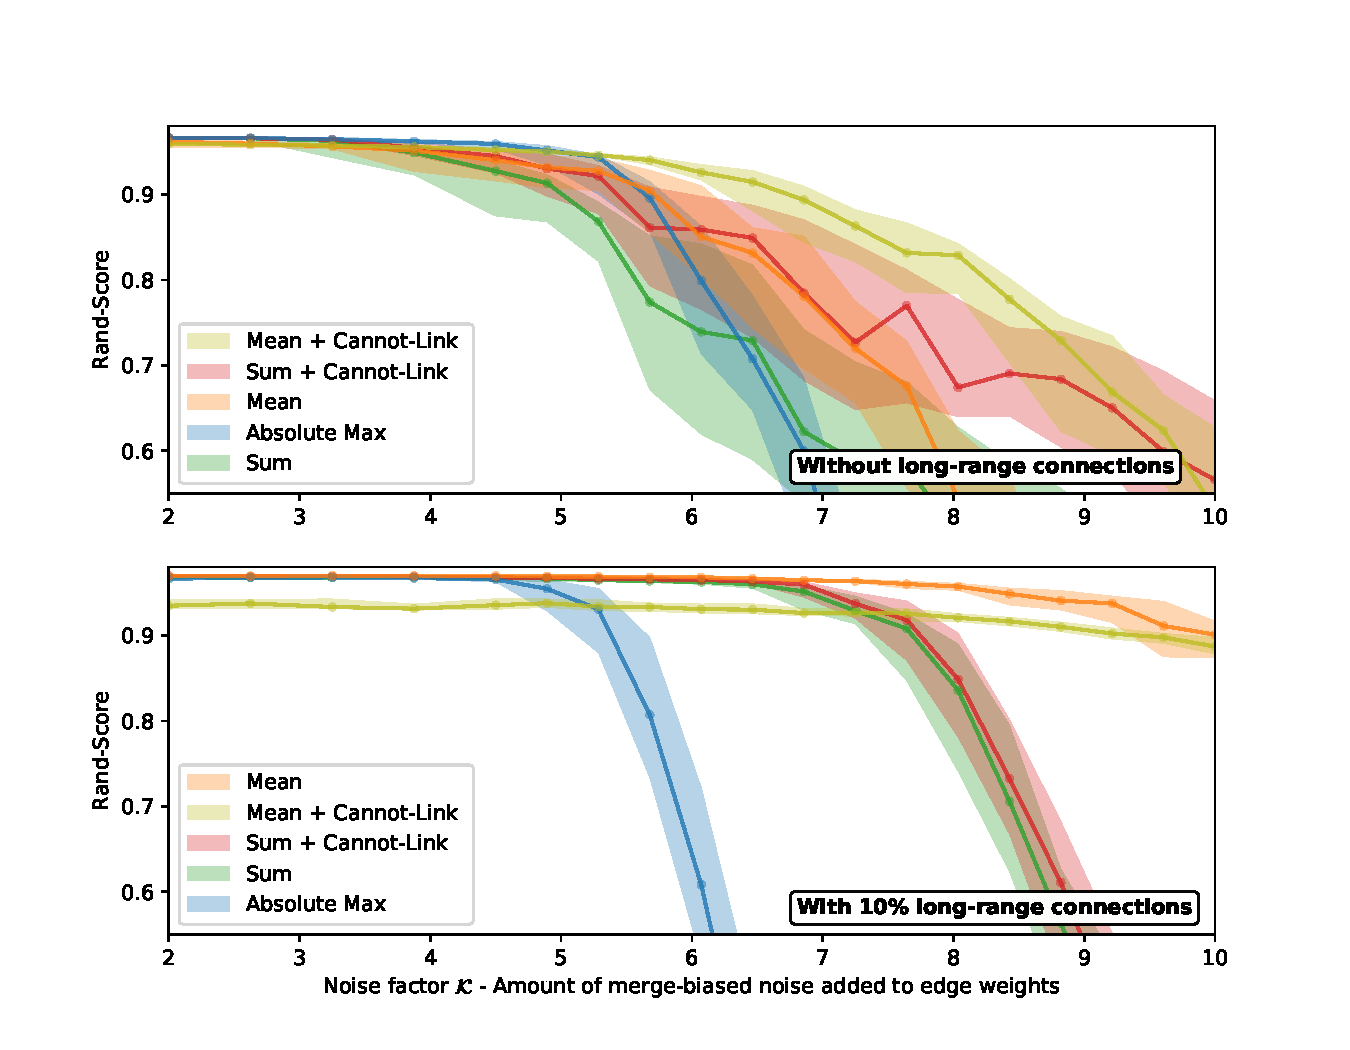
\includegraphics[width=0.50\textwidth,trim=0.35in 0.35in 0.35in 0.35in,clip]{./figs/merge_noise.pdf}
\caption{Plot illustrating results with merge-biased noise...}\label{fig:noise_merge}
\end{figure}


\subsection{Experimental setup and tested datasets}
\begin{itemize}
    \item Define long-range grid graph. (Mention the fact of enforcing local merge)
\item Introduce "Poisson" random graph with a given probability of long-range connections
\item Comment about the short- and long-range distinction in the MWS paper? It does not work that well in practice (applying post-processing to remove small segments is easier and better solution)
\item Define offset patterns (link to supplementary material), trained networks (loss, etc...) and setups on cremi and cityscapes 
\end{itemize}
